\section{Actividad}

\begin{frame}{Actividad}
    \textbf{Simulación estructural y electrónica del silicio.}

    \vspace{0.4cm}

    Objetivos:

    \begin{itemize}
        \item Optimización de ecutwfc
        \item Optimización de ecutrho
        \item Optimización de puntos k
        \item Optimización de parámetro de red
    \end{itemize}
\end{frame}

\begin{frame}
    \begin{figure}[H]
        \centering
        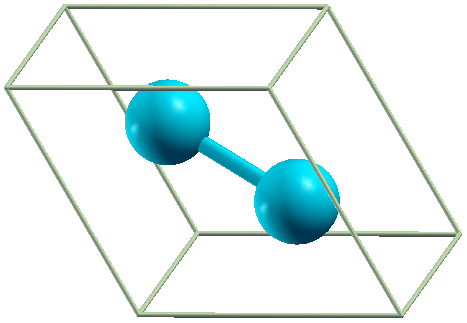
\includegraphics[scale=0.6]{images/silicene_cell.png}
        \caption{Celda unitaria del silicio.}
    \end{figure}
\end{frame}

\begin{frame}
    \textbf{Simulación estructural y electrónica del Siliceno.}

    \vspace{0.4cm}

    Objetivos:

    \begin{itemize}
        \item Optimización de puntos k
        \item Optimización de parámetro de red
        \item Cálculo de bandas
        \item Densidad de estados
    \end{itemize}
\end{frame}

\begin{frame}
    \begin{figure}[H]
        \centering
        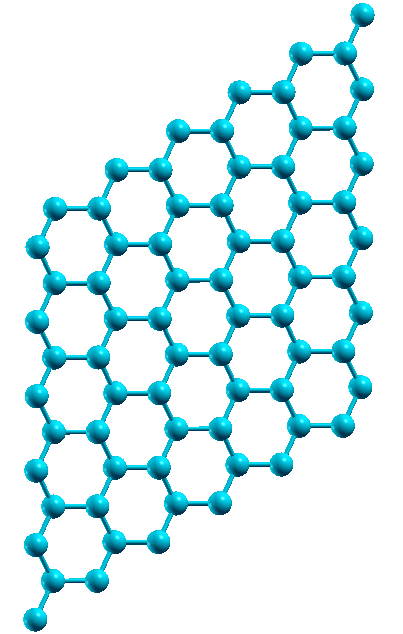
\includegraphics[scale=0.3]{images_siliceno/siliceno_2d.png}
        \caption{Celda unitaria del siliceno.}
    \end{figure}
\end{frame}

\begin{frame}
    \textbf{Simulación estructural y electrónica del Silicano.}

    \vspace{0.4cm}

    Objetivos:

    \begin{itemize}
        \item Optimización de ecutwfc
        \item Optimización de ecut
        \item Optimización de puntos k
        \item Optimización de parámetro de red
        \item Cálculo de bandas
        \item Densidad de estados
    \end{itemize}
\end{frame}

\begin{frame}
    \begin{figure}[H]
        \centering
        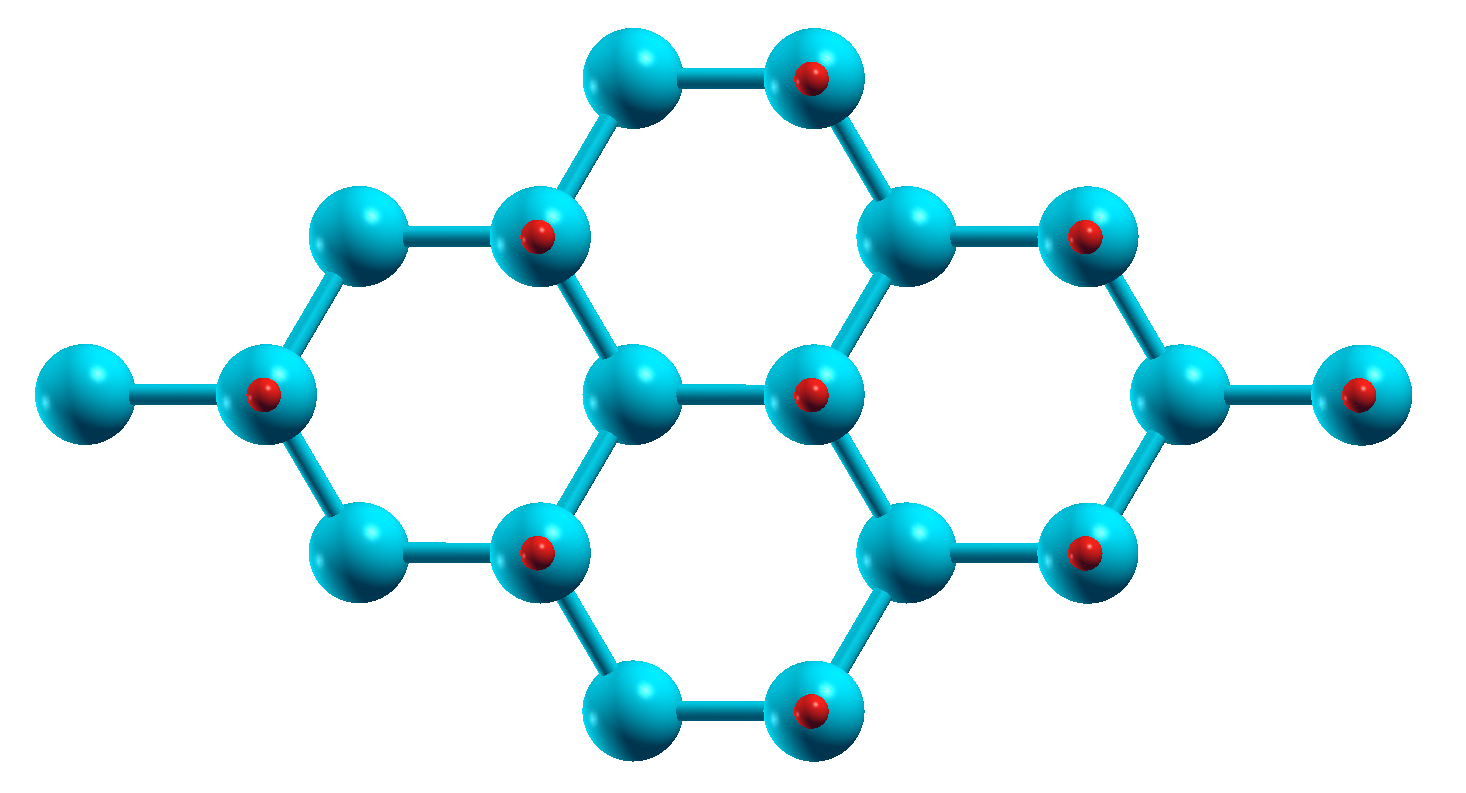
\includegraphics[scale=0.2]{images_silicano/silicano_structure.png}
        \caption{Celda unitaria del silicano.}
    \end{figure}
\end{frame}

\begin{frame}
    \begin{figure}[H]
        \centering
        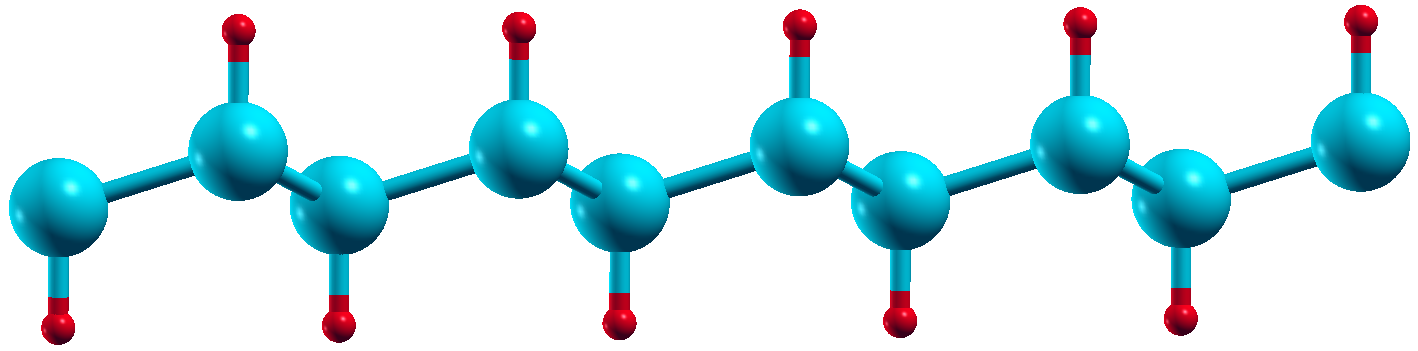
\includegraphics[scale=0.2]{images_silicano/silicano_structure_2.png}
        \caption{Celda unitaria del silicano.}
    \end{figure}
\end{frame}

\begin{frame}
    \textbf{ Silicio, siliceno y silicano.}

    \begin{itemize}
        \item Hacer una búsqueda en la literatura (artículos cientificos) de los parámetros 
            estructurales (parámetro de red, longitud de enlacee, ángulos) y propiedades
            electrónicas (estructura de bandas electrónicas, densidad de estados electrónicos)
            del silicio, siliceno y silicano.
    \end{itemize}
\end{frame}